\documentclass[{../../master}]{subfiles}
\graphicspath{{../..}}  % 個別コンパイル時の画像パスを解決する

\begin{document}

\section{\textsf{base\_link}の作成と追加}

節\ref{sec:create_urdf_package}までの作業で,ルートファイル\textsf{robot.xacro}の作成と\textsf{base\_footprint}リンクの定義を行いました.
この節ではロボットのボディのリンクである\textsf{base\_link}の定義とルートファイルへの追加の作業を行います.

\subsection{\textsf{base.xacro}の作成}

まず,\textsf{base\_link}の要素や属性の定義を記述するファイルを作成します.
\textsf{urdf/}ディレクトリ以下に\textsf{base/}ディレクトリを作成し,\textsf{base.xacro}という名前のファイルを作成します.
そして,まずはコード\ref{code:base_link_first_step}のような内容を記述します.

\begin{lstlisting}[language=XML, caption=\textsf{base.xacro}, label=code:base_link_first_step]
<?xml version="1.0"?>
<robot xmlns:xacro="http://ros.org/wiki/xacro">
  <xacro:macro name="base" params="parent *joint_origin">
    
  </xacro:macro>
</robot>
\end{lstlisting}

ルートファイルと同じく,\textsf{robot}タグをトップレベルに記述し,その中に他の全ての要素を記述していきます.
ただし,コンポーネントファイルには\textsf{name}属性を書く必要はありません.名前空間だけ指定しておきましょう.

\textsf{robot}タグの中には,\textsf{xacro:macro}タグが書かれています.
これが\textsf{xacro}におけるマクロの定義であり,ルートファイルから呼び出されるものです.
マクロの中に\textsf{link}や\textsf{joint}等のタグを記述しておけば,ルートファイルから呼び出されたときにそれらが展開される,という仕組みです.
\textsf{xacro:macro}タグには\textsf{name}属性と\textsf{params}属性があります.
\textsf{name}属性にはマクロの名前を指定します.
\textsf{params}属性には,そのマクロが取る引数を指定することができます.
引数は複数設定することができ,半角スペースで区切って記述します.
コード\ref{code:base_link_first_step}では,引数として\textsf{parent}(親リンク名の指定)と\textsf{*joint\_origin}
\footnote{アスタリスクが先頭に付くパラメータは「ブロックパラメータ」と呼ばれるパラメータで,任意の要素を展開することができます.}
(座標原点の指定)の2つを取るように設定しています.

\textsf{base.xacro}ファイルでは,このマクロを読み込んだら「\textsf{base\_link}の定義」と「\textsf{base\_footprint}と\textsf{base\_link}を繋ぐジョイント\textsf{base\_link\_joint}の定義」が行われるようにマクロを定義します.

\subsection{\textsf{joint}の設定}

この小節では\textsf{base\_link\_joint}の定義を行います.
コード\ref{code:base_link_joint_configuration}のようにマクロタグ内に\textsf{joint}タグを追記します.

\begin{lstlisting}[language=XML, caption=Configurate \textsf{base\_link\_joint}, label=code:base_link_joint_configuration]
<?xml version="1.0"?>
<robot xmlns:xacro="http://ros.org/wiki/xacro">
  <xacro:macro name="base" params="parent *joint_origin">
    <joint name="base_link_joint" type="fixed">
      <xacro:insert_block name="joint_origin"/>
      <parent link="${parent}"/>
      <child link="base_link"/>
    </joint>
  </xacro:macro>
</robot>
\end{lstlisting}

\textsf{joint}タグは\textsf{name}と\textsf{type}の2つの属性を持ち,また以下の要素を持ちます.\cite{urdf_xml_joint}

\begin{itemize}
  \item \textsf{origin}:親リンクから見たジョイントの原点座標
  \item \textsf{parent}:親リンク名
  \item \textsf{child}:子リンク名
  \item \textsf{axis}:ジョイントの軸.回転ジョイントの場合は回転軸を表す
  \item \textsf{calibration}:ジョイントの絶対位置を校正するために使用される,ジョイントの基準位置
  \item \textsf{dynamics}:ジョイントの物理的特性を指定するための要素
  \item \textsf{limit}:ジョイントの角度,力,速度のリミットを指定するための要素
  \item \textsf{mimic}:他のジョイントの動きを真似させるときに使用する要素
  \item \textsf{safety\_controller}:ジョイントが安全に動作するために設定するソフトなリミット
\end{itemize}

\noindent
このうち,ジョイントの定義に必須なのは\textsf{parent}と\textsf{child}のみで,他の要素は指定しなくてもジョイントを定義することができます.

ここでは,ジョイント名を「\textsf{base\_link\_joint}」,ジョイントタイプを「\textsf{fixed}」とし,要素には\textsf{parent}と\textsf{child},そして\textsf{origin}を設定します.

\textsf{child}要素は\textsf{base\_link}です.
\textsf{base\_link}はまだ存在せず,\ref{sec:base_link_define_link_tag}で定義します.
\textsf{parent}要素にはマクロが引数として受け取った値をそのまま使用します.
引数をマクロ内で利用するには,\textsf{\$\{\<PARAMETER\_NAME\>\}}の書式を使用します.

\textsf{joint}タグの\textsf{origin}要素で指定するのは,親リンクから見たジョイントの原点座標です.
図\ref{fig:joint}のように,ジョイントが子リンクの原点になります.
ここでは\textsf{base\_link}が子リンクなので,\textsf{base\_link}の座標系原点は\textsf{base\_link\_joint}の位置になるという事になります.

\begin{figure}[ht]
  \centering
  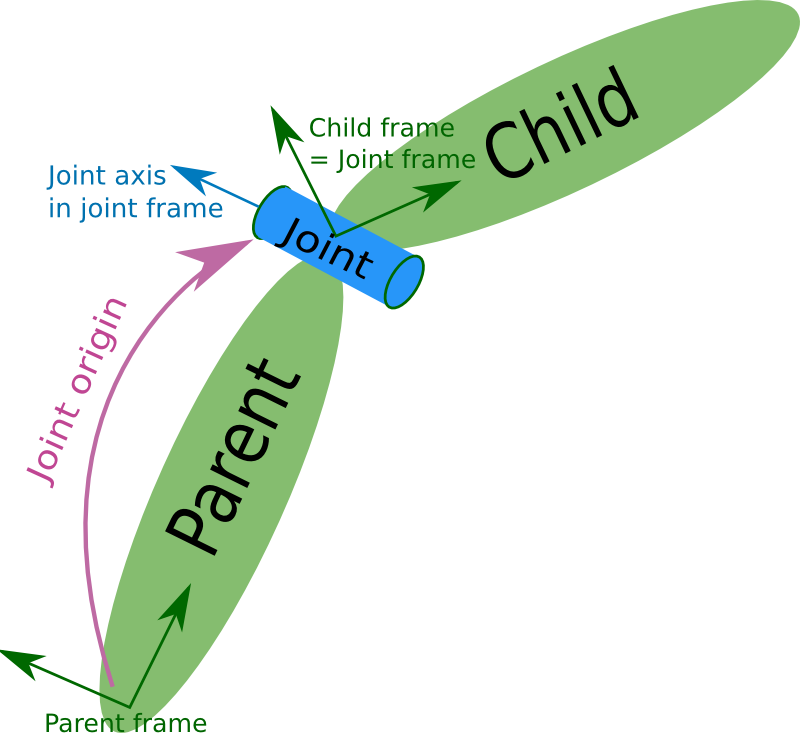
\includegraphics[width=100truemm, clip]{images/joint.png}
  \caption{Coordinate Transformation Relationship Between Link and Joint\cite{urdf_xml_joint}}
  \label{fig:joint}
\end{figure}

\textsf{origin}要素もマクロが引数として受け取ったものを使用します.
ただし,\textsf{origin}要素は単なる値ではないため,\textsf{parent}要素のようにそのまま使うことはできません.
そこで使用するのがブロックパラメータと呼ばれる引数です.
これを使用することで,ルートファイルからジョイントの\textsf{origin}要素を定義できるようになります.
コード\ref{code:base_link_joint_configuration}では\textsf{*joint\_origin}という名前でブロックパラメータを定義しています.
ルートファイルから読み込む際の詳細は\label{sec:base_link_include}で説明します.

ジョイントの設定は以上で完了です.次は\textsf{link}タグの設定を行います.

\subsection{\textsf{link}タグの設定}
\label{sec:base_link_define_link_tag}

ここから\textsf{link}タグを定義して,\textsf{base\_link}の要素を記述していきます.
\textsf{link}タグは\textsf{inertial},\textsf{visual},\textsf{collision}の3つの要素を持ちます.
\textsf{link}タグ及び各要素の詳細について知りたい方は,ROS Wikiのページ\footnote{\url{http://wiki.ros.org/urdf/XML/link}}を参照してください.

Gazeboシミュレーションを行う際は全ての要素について定義する必要がありますが,\textsf{rviz}で可視化するだけなら\textsf{visual}要素を設定するだけで事足ります.
本章では実機用URDFの記述を目的としているため,ここではシミュレーション用の設定については説明しません.
シミュレーション用の設定については後の章で解説します.

\textsf{visual}要素はモデルの見た目の要素を定義するタグです.
コード\ref{code:base_link_link_tag_element}のようにマクロタグ内に\textsf{link}タグを追記し,更にその中に\textsf{visual}要素を記述します.

\begin{lstlisting}[language=XML, caption=\textsf{link} Element, label=code:base_link_link_tag_element]
<?xml version="1.0"?>
<robot xmlns:xacro="http://ros.org/wiki/xacro">
  <xacro:macro name="base" params="parent *joint_origin">
    <joint name="base_link_joint" type="fixed">
      <xacro:insert_block name="joint_origin"/>
      <parent link="${parent}"/>
      <child link="base_link"/>
    </joint>

    <link name="base_link">
      <visual>
        <origin xyz="0.0 0.0 0.0"/>
        <geometry>
          <mesh filename="package://adamr2_description/meshes/base_link.STL"/>
        </geometry>
        <material name="red">
          <color rgba="1.0 0.0 0.0 1.0"/>
        </material>
      </visual>
    </link>
  </xacro:macro>
</robot>
\end{lstlisting}

\textsf{visual}要素は更に\textsf{origin},\textsf{geometry},\textsf{material}要素を持ちます.
\textsf{geometry}要素ではリンクの見た目を表す形状を定義します.
長方形,球,円柱等のプリミティブな図形を設定できる他,STLファイルを読み込んで設定することができます.
実際,コード\ref{code:base_link_link_tag_element}では\textsf{mesh}要素にSTLファイルを指定して形状を設定しています.
STLファイルは\ref{sec:base_link_create_mesh_file}で作成します.

\textsf{origin}要素では\textsf{geometry}要素で指定した図形の原点の座標を設定することができます.
リンクの座標系から見た位置,即ちこのリンクが所属するジョイントの原点からみた位置で指定することになります.
このドキュメントでは,基本的にリンクの位置は\textsf{joint}タグの位置を設定することで決定します.
そのため,\textsf{link}タグの\textsf{origin}要素の値はほとんどの場合でゼロになります.

\textsf{material}要素ではリンクの色を設定することができます.
ただし,プリミティブ図形またはSTLファイルを使用する場合は,単色でしか設定できません.
リンクの見た目の色を詳細に決定したい場合は,COLLADAファイル(拡張子は\textsf{*.dae})を用意する必要があります.
ロボットの開発にとってあまり本質的ではないと考えたので,このドキュメントではCOLLADAファイルの作成については説明しません.

\subsection{メッシュファイル(STL形式)の作成と割り当て}
\label{sec:base_link_create_mesh_file}

\textsf{visual}要素の\textsf{mesh}に指定するSTLファイルを,3D-CADソフトであるSolidWorks2019を用いて作成します.
SolidWorksにはパーツファイルをSTLにエクスポートする機能があるので,これを使います.

ROS REP:103\footnote{\url{https://www.ros.org/reps/rep-0103.html}}にあるように,ROSでは長さの単位を全てメートルで扱います.
しかし,3D-CADで設計を行うときはミリメートル単位でモデリングするのが一般的です.
従って,そのままSTLエクスポートすると,ROSから読み込んだときにモデルの大きさが1000倍になってしまいます.
また,ROSではロボットの座標軸の向きは「X軸がロボットの前進方向,Z軸は鉛直上向き方向,Y軸は右手座標系となるような向き」と決められています.
3D-CADのデフォルト座標軸がこのような向きになっていることは少ないため,STLファイルをエクスポートした後にBlender等の3D-CGファイルでスケールや向きを調整しなければならない場合が殆どです.

しかし,SolidWorksにはSTLファイルをエクスポートする際に,単位系や座標系を指定することができる機能があります.
そのため,適切な設定を行いさえすれば3D-CGソフトで後処理を行うことは必要ありません.

図\ref{fig:base_link_cad_model}に,\textsf{base\_link}に対応付けるロボットのボディの3D-CADモデルを示します.
これはアセンブリファイルをパーツファイルに変換したもので,筐体の他,アクチュエータ(ホイールは含まない)も内包しています.
3D-CADの座標軸が図の左下に表示されていますが,X軸はロボットの前方を向いているものの,Z軸が鉛直上向きになっていません.
また,ミリメートル単位で設計を行ったため,単位変換を行う必要があります.

\begin{figure}[ht]
  \centering
  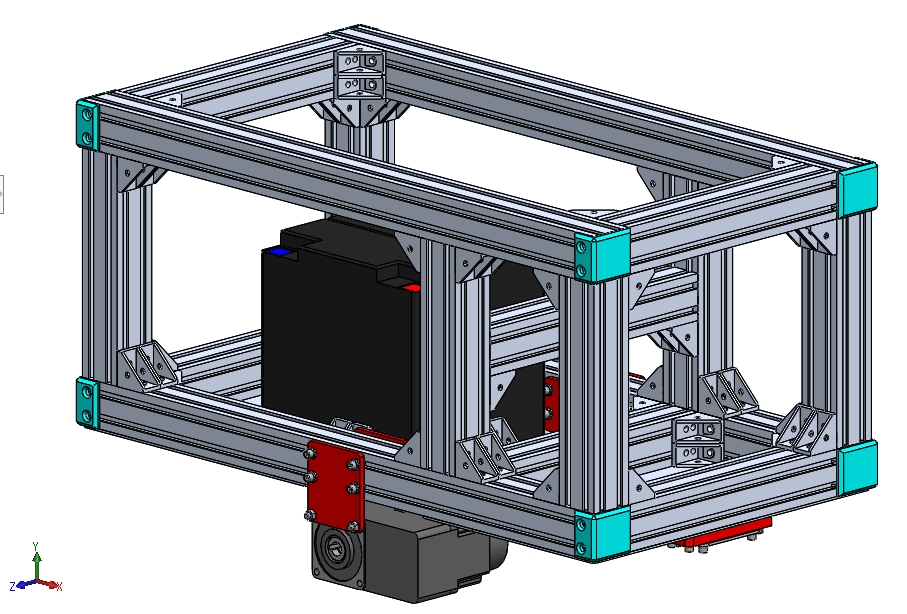
\includegraphics[width=100truemm, clip]{images/base_link_cad_model.png}
  \caption{3D Model of \textsf{base\_link}}
  \label{fig:base_link_cad_model}
\end{figure}

STLファイルをエクスポートする前の準備として,まず座標系を定義しましょう.
今回のモデルでは,原点はアルミフレームが描く直方体の中心に位置しているので,STLファイルの原点にしたい場所に新たに点を打つ必要はありません.
まずは座標系のもとになる軸を定義します.フィーチャー$\rightarrow$参照ジオメトリ$\rightarrow$軸を選択します.
そして,図\ref{fig:base_link_create_axes}のように2つの平面を選択して,X軸,Y軸,Z軸の3本を新たに定義します.

\begin{figure}[ht]
  \centering
  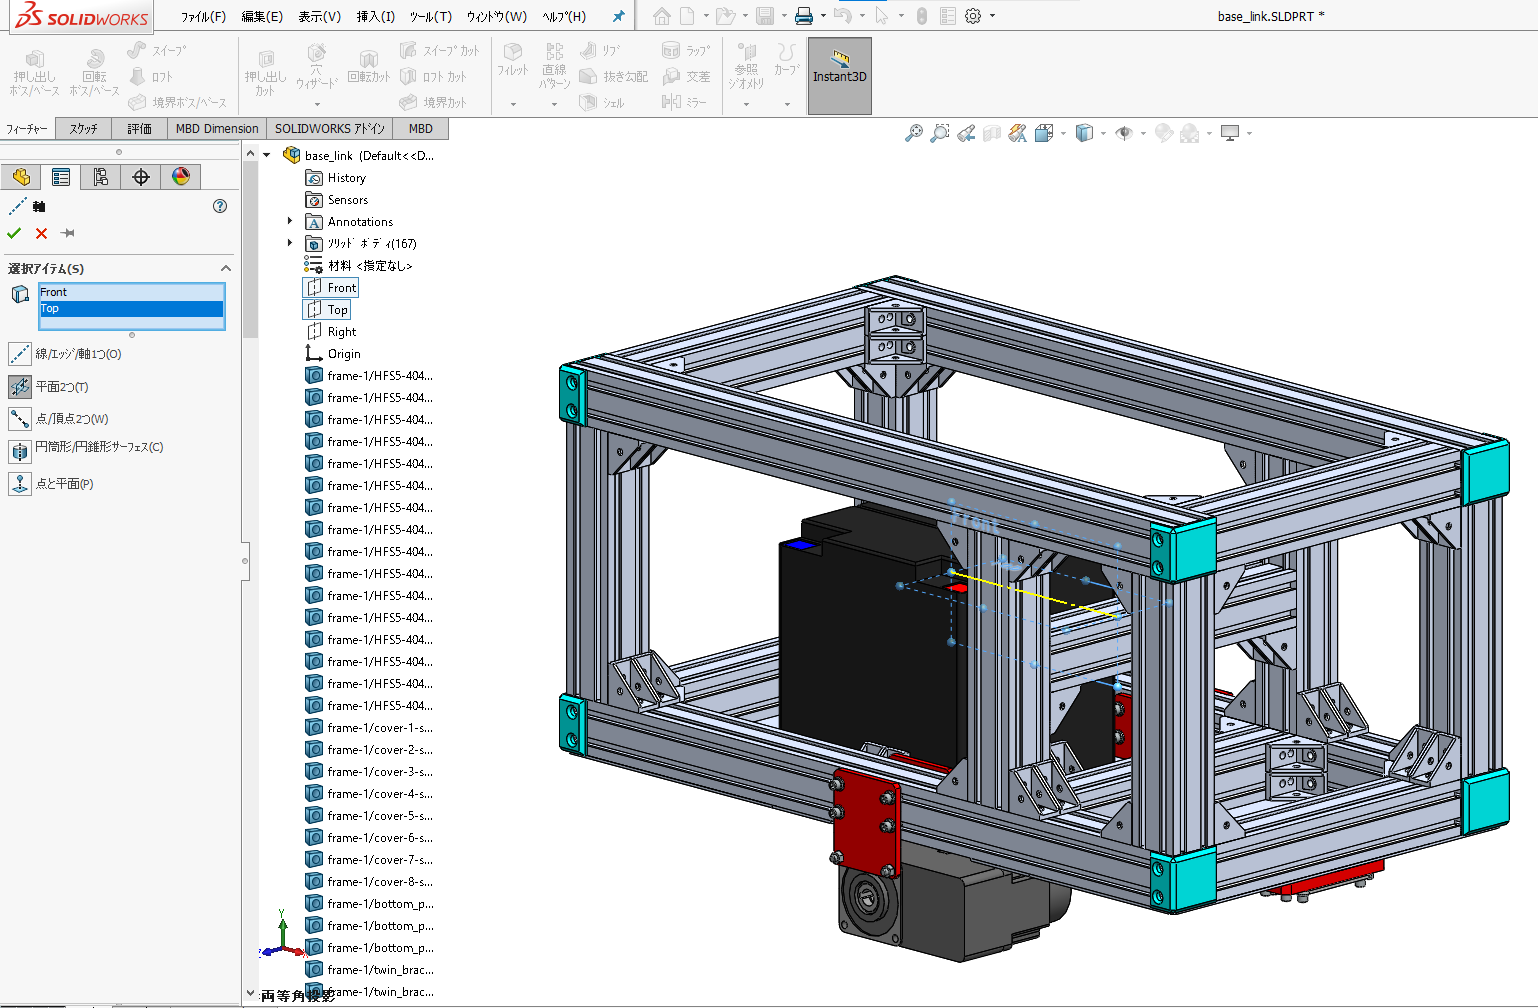
\includegraphics[width=100truemm, clip]{images/base_link_create_axes.png}
  \caption{Add Axes for STL Export}
  \label{fig:base_link_create_axes}
\end{figure}

\noindent
軸を追加したら,座標系を定義します.
先ほど追加した軸を使って,ROSが推奨する座標軸の向きになるように設定します.
少し見づらいですが,図\ref{fig:base_link_create_coordinate_system}ではX軸に軸1を,Z軸に軸3を対応付けた結果,望ましい座標軸の向きになっていることがわかります.

\begin{figure}[ht]
  \centering
  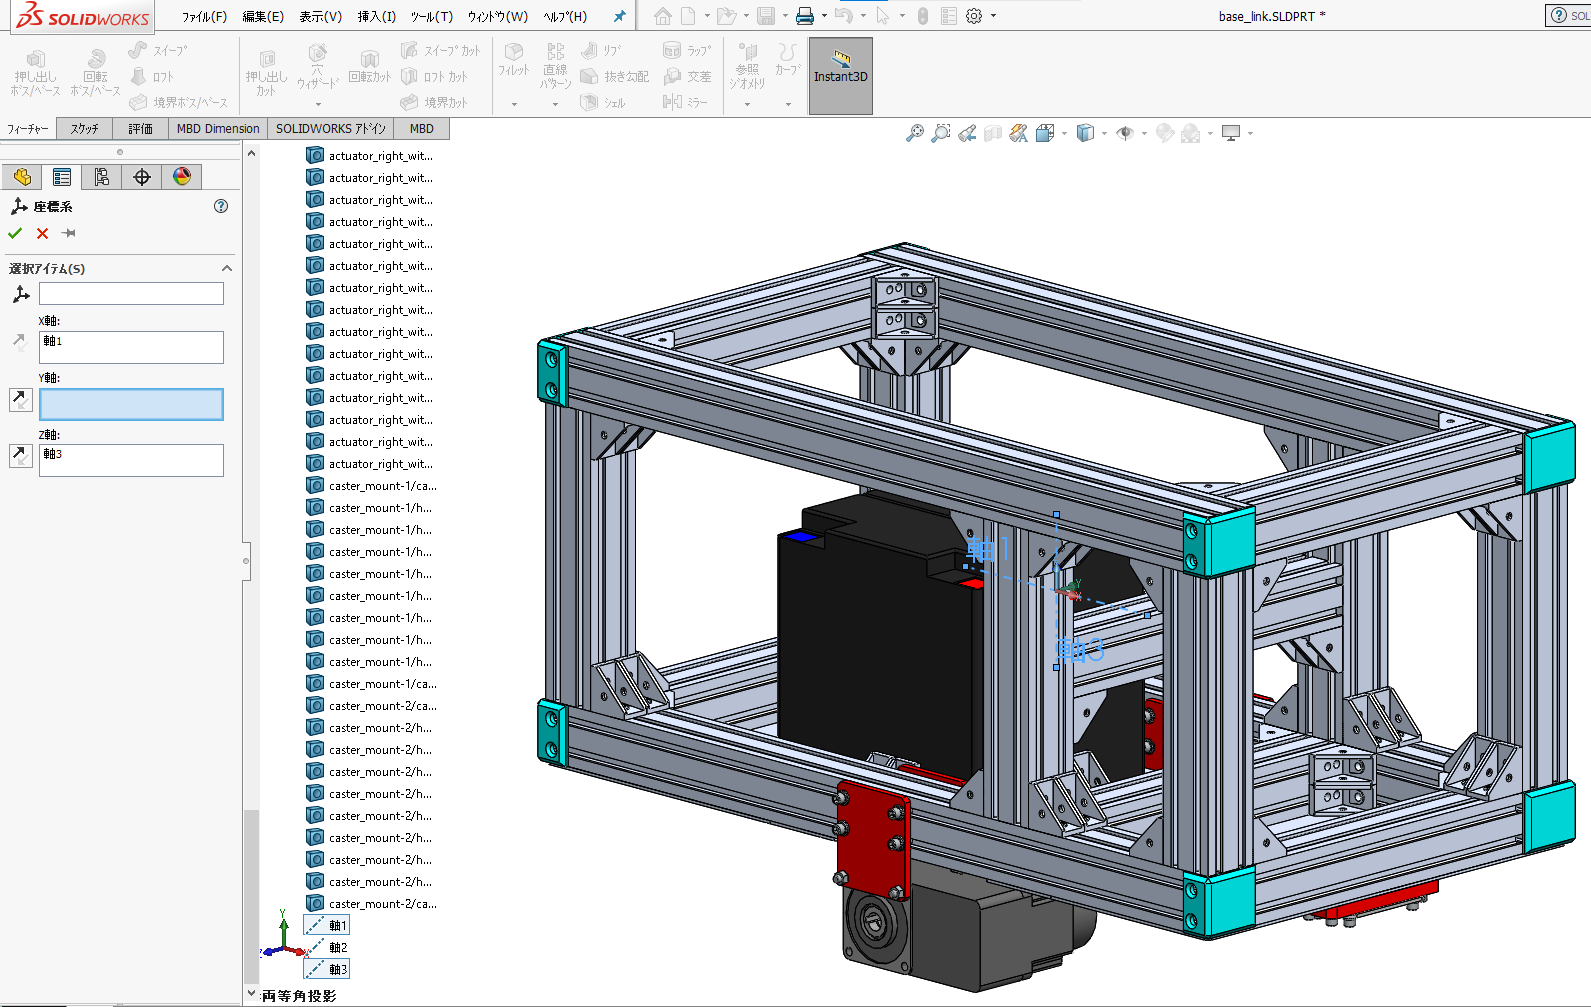
\includegraphics[width=100truemm, clip]{images/base_link_create_coordinate_system.png}
  \caption{Add Coordinate System for STL Export}
  \label{fig:base_link_create_coordinate_system}
\end{figure}

座標系の定義ができたので,STLファイルをエクスポートしましょう.
指定保存を開き,ファイルの種類(拡張子)に「STL」を選択します.
STLを選択すると,「オプション」ボタンが表示されるので,それをクリックします.

\begin{figure}[ht]
  \centering
  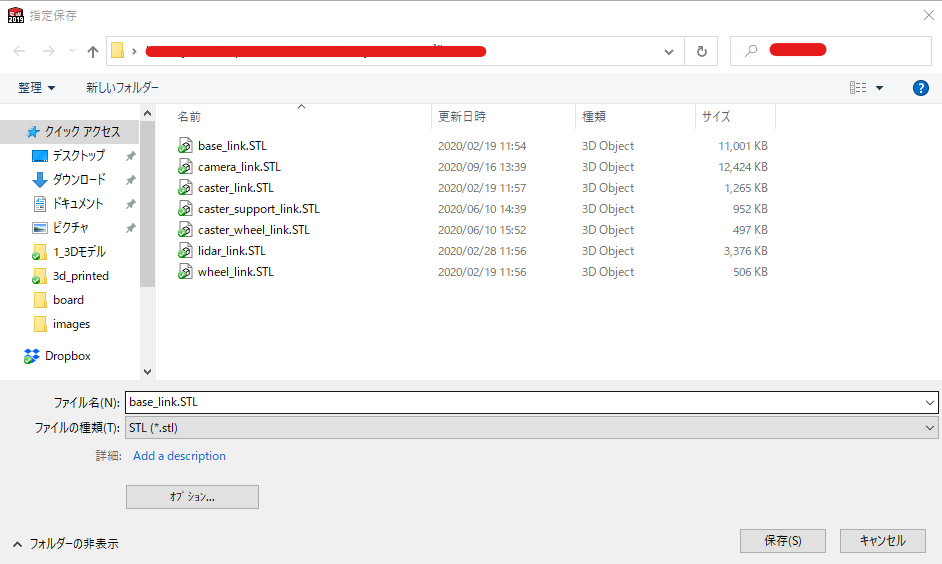
\includegraphics[width=100truemm, clip]{images/base_link_save_as_stl.png}
  \caption{Save as STL File}
  \label{fig:base_link_save_as_stl}
\end{figure}

\noindent
オプションを開くと,図\ref{fig:base_link_stl_export_options}のような画面が表示されます.
ここで単位と出力座標系を設定します(\ref{fig:base_link_stl_export_options}で赤線を引いたところ).
単位をメートルに,出力座標系に先ほど作成した座標系(ここでは「座標系1」という名前)を設定し,「モデルの座標系で出力」というチェックボックスをオンにします.
お好みで解像度の設定もできます.「粗表示」を選ぶとモデルが粗くなってしまいますが,ファイルの容量を減らすことができます.

\begin{figure}[ht]
  \centering
  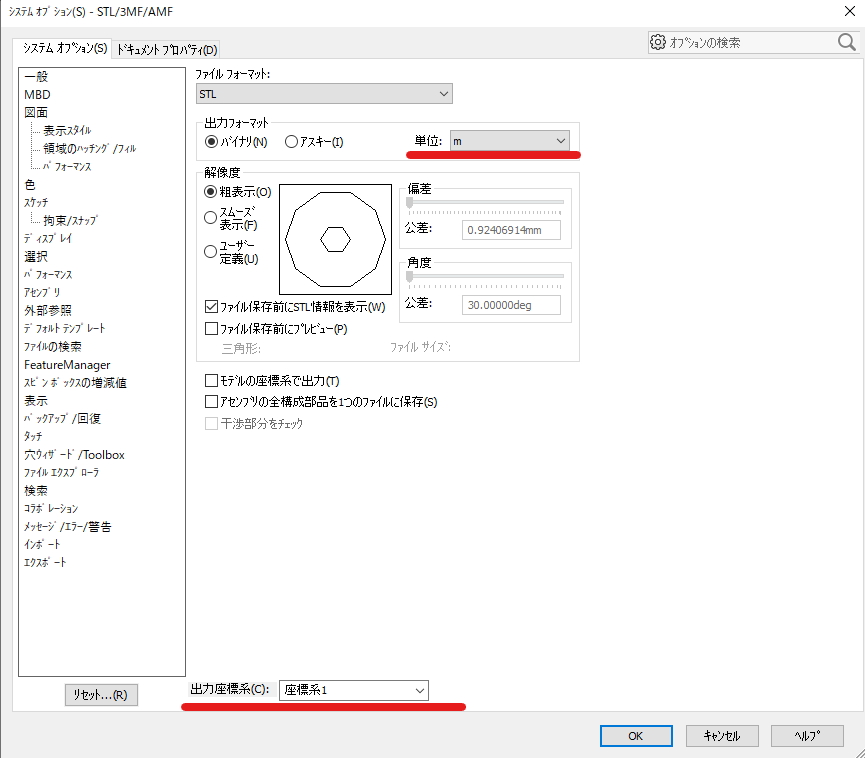
\includegraphics[width=100truemm, clip]{images/base_link_stl_export_options.png}
  \caption{STL Export Options}
  \label{fig:base_link_stl_export_options}
\end{figure}

この設定で「OK」をクリックし,「保存」を選択することで,ROSでそのまま使用できるSTLファイルを作成することができます.
このSTLファイルを,\textsf{adamr2\_description/meshes/}ディレクトリに\textsf{base\_link.STL}という名前で保存します.
コード\ref{code:base_link_link_tag_element}が正しく記述されていれば,STLファイルを読み込むことができるようになります.

\subsection{ルートファイルからインクルードする}
\label{sec:base_link_include}

ここまでの作業で\textsf{base\_link}の定義を完了することができたので,これをルートファイルから読み込んでロボットモデルに組み込みましょう.
コード\ref{code:robot_xacro_add_base_link}に,\textsf{robot.xacro}にいくつかの文を追記します.

\begin{lstlisting}[language=XML, label=code:robot_xacro_add_base_link, caption=Add \textsf{base\_link} to Robot Model]
<?xml version="1.0"?>
<robot name="adamr2" xmlns:xacro="http://ros.org/wiki/xacro">
  <xacro:include filename="$(find adamr2_description)/urdf/base/base.xacro"/>

  <link name="base_footprint"/>

  <xacro:base parent="base_footprint">
    <origin xyz="0.0 0.0 0.262"/>
  </xacro:base>

</robot>
\end{lstlisting}

3行目に追記したコマンド\textsf{xacro:include}で,\textsf{base.xacro}ファイルを読み込んでいます.
これにより,\textsf{base.xacro}で定義したマクロを使用できるようになります.
そして,7行目から9行目で\textsf{xacro:base}マクロを使って\textsf{base\_link}と\textsf{base\_link\_joint}を定義しています.
マクロタグ内で\textsf{origin}要素の記述を行っているのは,マクロがブロックパラメータとして\textsf{origin}要素を引数としているからです.
こうすることにより,設計変更が発生してリンクの場所を変更しなければならなくなっても,\textsf{robot.xacro}を編集するだけで対応することが出来るようになります.

\textsf{robot.xacro}を編集したら,念の為URDFチェックをしておきましょう.
URDFの構文チェックの手順は,\ref{sec:urdf_check}の手順を参照してください.
URDFを正しく記述できていれば,コード\ref{code:base_link_check_urdf_result}のように表示されるはずです.

\begin{lstlisting}[language=sh, label=code:base_link_check_urdf_result, caption=Result of Check URDF]
robot name is: adamr2
---------- Successfully Parsed XML ---------------
root Link: base_footprint has 1 child(ren)
    child(1):  base_link  
\end{lstlisting}

\subsection{\textsf{rviz}による可視化}
\label{sec:base_link_visualize_by_rviz}

せっかくリンクを追加したので,\textsf{rviz}で可視化してみましょう.
\textsf{launch/}ディレクトリを作成し,その中に\textsf{rviz}を起動するためのlaunchファイル\textsf{display.launch}を作成し,コード\ref{code:base_link_display_launch}の内容を記述します.

\begin{lstlisting}[language=XML, label=code:base_link_display_launch, caption=\textsf{display.launch}]
<launch>
  <arg name="model" default="$(find adamr2_description)/urdf/robot.xacro"/>

  <param name="robot_description" command="$(find xacro)/xacro $(arg model)"/>

  <node name="robot_state_publisher" pkg="robot_state_publisher" type="robot_state_publisher"/>
  <node name="rviz" pkg="rviz" type="rviz"/>
</launch>
\end{lstlisting}

\textsf{param}タグで\textsf{robot.xacro}を展開し,\textsf{robot\_description}という名前のパラメータに登録します.
ROSではロボットのリンクやジョイントの状態を,\textsf{robot\_description}という名前のパラメータで一元管理しています.
URDFの情報をこのパラメータに登録することで,URDFで定義したロボットのモデルをROSに伝えます.

また,このlaunchファイルでは2つのノードを起動しています.
1つは\textsf{robot\_state\_publisher}ノードです.このノードは\textsf{robot\_description}パラメータの情報を解釈してTFを投げてくれるノードです.
2つ目は\textsf{rviz}です.

launchファイルを作成したら,一旦パッケージをビルドしておきましょう.
パッケージをビルドすることで,そのパッケージにlaunchファイルが存在することをシステムに登録できます.
\footnote{ROS1では,ROS2のようにlaunchファイルを変更する度にビルドする必要はありません.ここでの作業はlaunchファイルの存在をシステムに知らせるためのものです.}
ROSのワークスペースに移動して,コード\ref{code:adamr2_description_build_package}のコマンドを実行します.

\begin{lstlisting}[language=sh, label=code:adamr2_description_build_package, caption=Build \textsf{adamr2\_description} Package]
cd ~/catkin_ws/src
catkin build adamr2_description
source ~/catkin_ws/devel/setup.bash 
\end{lstlisting}

パッケージをビルドしたら,launchファイルを実行してみましょう.

\begin{lstlisting}[language=sh, caption=Launch \textsf{display.launch}]
roslaunch adamr2_description display.launch
\end{lstlisting}

launchファイルを実行すると,\textsf{rviz}が起動し,図\ref{fig:plain_rviz}のような画面が表示されます.

\begin{figure}[ht]
  \centering
  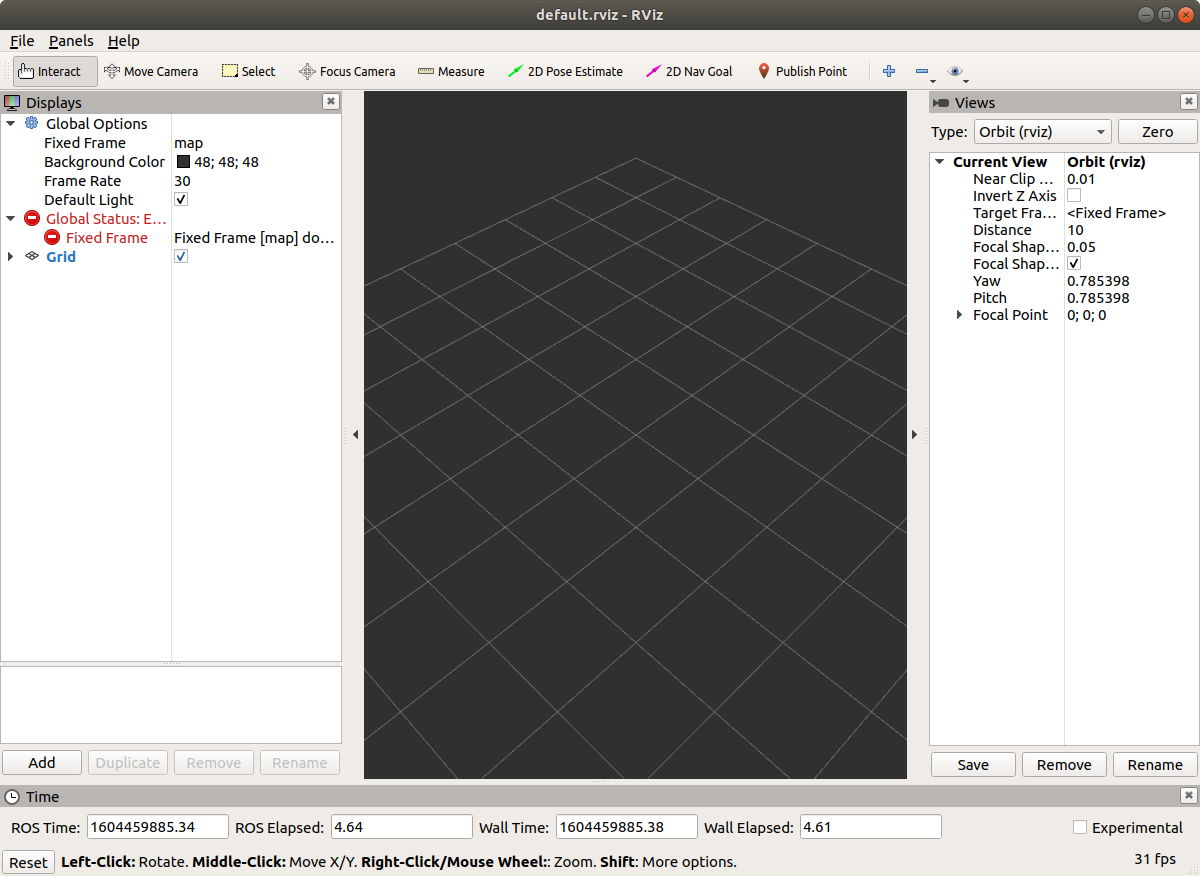
\includegraphics[width=100truemm]{images/plain_rviz.png}
  \caption{Screenshot of \textsf{rviz} Right After It Started}
  \label{fig:plain_rviz}
\end{figure}

起動した直後はオプションを何も設定していないので,何も表示されません.
ロボットのモデルを表示するためには,左下の「Add」ボタンを押し,「\textsf{RobotModel}」を追加します(図\ref{fig:rviz_add_robot_model}).

\begin{figure}[ht]
  \centering
  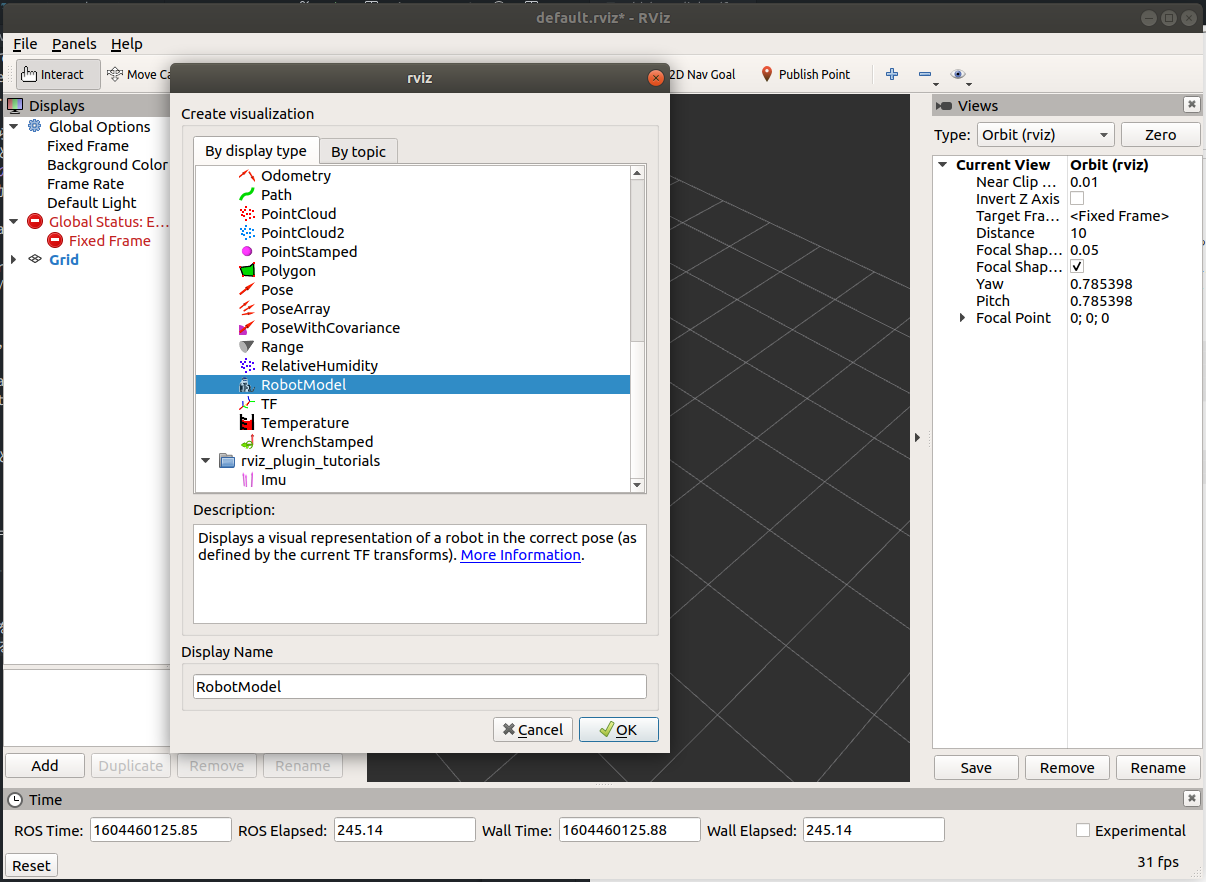
\includegraphics[width=100truemm]{images/rviz_add_robot_model.png}
  \caption{Add \textsf{RobotModel} to \textsf{rviz}}
  \label{fig:rviz_add_robot_model}
\end{figure}

\noindent
そして,\textsf{Fixed Frame}の値を\textsf{base\_footprint}に変更します.
デフォルトの値は\textsf{map}というフレームが割り当てられていますが,ロボットのモデルには\textsf{map}というフレームは存在しません.
ロボットモデルのルートとなるフレーム名は\textsf{base\_footprint}に設定しているので,プルダウンメニューを開き,\textsf{base\_footprint}を選択します.

ここまで設定すれば,図\ref{fig:rviz_robot_model_subccessfully_viewed}のようにロボットのモデルが正しく表示されるはずです.
\textsf{base\_link}がホイールの大きさを考慮した高さに置かれていることが分かると思います.

\begin{figure}[ht]
  \centering
  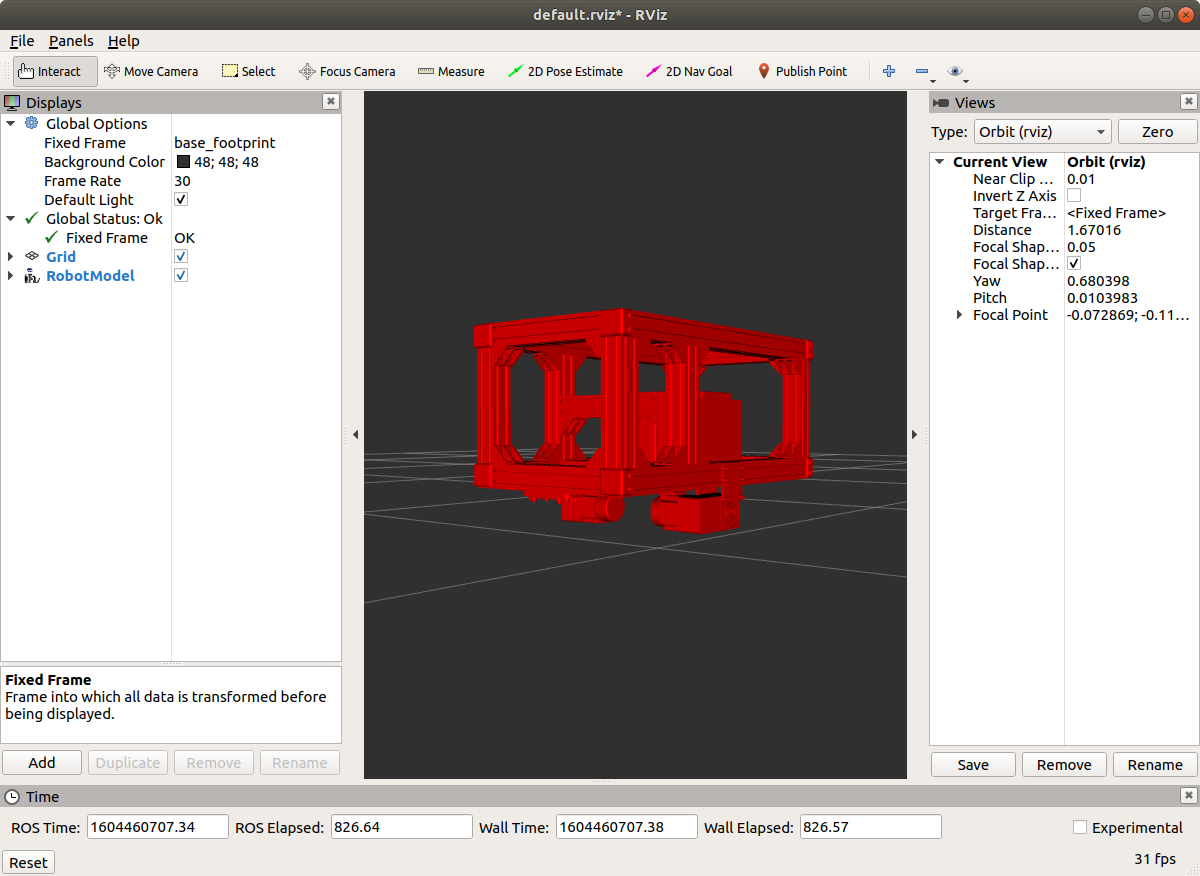
\includegraphics[width=100truemm]{images/rviz_robot_model_successfully_viewed.png}
  \caption{\textsf{base\_link} is Correctly Displayed}
  \label{fig:rviz_robot_model_subccessfully_viewed}
\end{figure}

本節では,コンポーネントとしてのxacroファイルの記述の仕方,SolidWorksを利用したSTLファイルの作成方法,ルートファイルからのインクルードの仕方,及び\textsf{rviz}を使ったURDFモデルの可視化について説明しました.
センサやホイール等のコンポーネントも,本節で説明した手順の通りに追加することができます.
次節以降の作業を行う際にづまづいたときは,本節に戻って手順を確認してください.

\end{document}